% Chapter 2 - Absorptive Capacity


%That said, a recent study by \citet{soda2017harvesting} found the efforts of those who practice \emph{tertius inungens brokerage} often go unrecognised or under-appreciated. Building consensus while keeping together a broad, diverse, and loosely connected coalition may incur steep coordination costs. Such costs might dilute the structural advantages of being a broker and make it more difficult to win recognition and agreement from network alters.

\section{Introduction}

Despite the vast body of research that has examined the characteristics and consequences of absorptive capacity, the concept remains elusive for researchers and practitioners \citep{duchek2013capturing,omidvar2013revisiting}. Efforts to understand how absorptive capacity contributes to firm performance have been confounded by different conceptualisations, questionable assumptions, and inconsistent findings from empirical research \citep{lane2006reification,lichtenthaler2016absorptive}. Additionally, absorptive capacity is becoming more grounded thanks to the growing adoption of open innovation as a competitive strategy \citep{volberda2010perspective,ahn2016beyond,xia2016unpacking}. Figure \ref{fig:bibliometric} shows that the academic interest in absorptive capacity has continued to grow exponentially. Though research into open innovation has increased, the influence of tacit knowledge on absorptive capacity and open innovation appears to be a neglected area of research.\medskip 

\begin{figure}
	\small
	\centering
	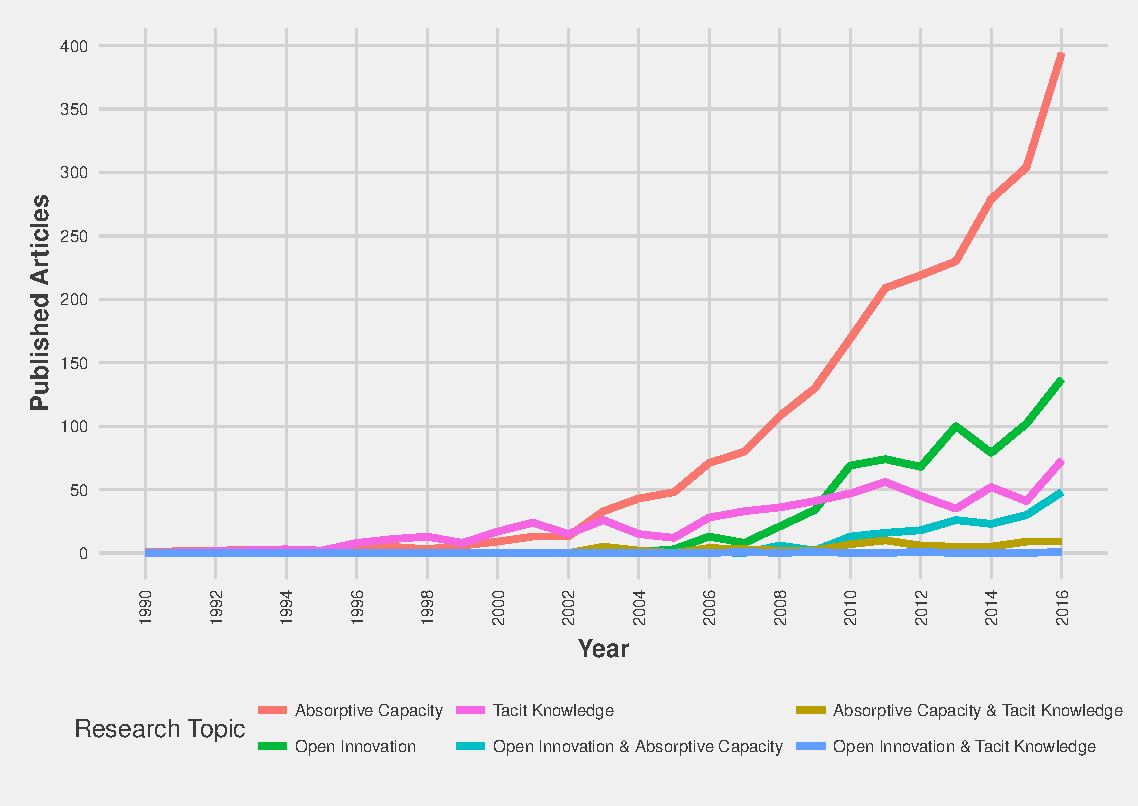
\includegraphics[width=1.0\linewidth]{Images/bibliometric}
	\caption{Research articles published per year. Data from Thomson Reuters Web of Science\texttrademark.}
	\label{fig:bibliometric}
\end{figure}

This chapter explores the multidimensional nature of absorptive capacity and how this relates to open innovation. Attention is given to the role of tacit knowledge in absorptive capacity processes and delivering open innovation success. \medskip

\section{Relative differences in absorptive capacity} 

The term \enquote{absorptive capacity} was introduced by \citet{cohen1989innovation}, who referred to the ability of a firm to acquire, assimilate and exploit knowledge from the environment as its \enquote{learning} or \enquote{absorptive} capacity. They formalised the concept in a seminal paper the following year in which they defined absorptive capacity as the \enquote{ability of a firm to recognise the value of new, external information, assimilate it, and apply it to commercial ends} \citep{cohen1990absorptive}. They embraced a cognitive approach to absorptive capacity by connecting ideas from individual learning to organisations. Similar to individuals, firms have memories that can be used to accumulate or stockpile knowledge. \citet{cohen1990absorptive} emphasised the importance of prior related knowledge because it facilitates associative learning in which events are recorded into memory by establishing connections with pre-existing concepts. According to them, the amount of prior related knowledge that a firm can accumulate determines its absorptive capacity. \medskip

\citet{cohen1990absorptive} addressed absorptive capacity in absolute terms. They implied that firms with absorptive capacity are equally capable of learning from all other organisations. To them, knowledge is something that exists in the environment and all that a firm needs to do is discover and apply it \citep{omidvar2013revisiting}. \citet{lane1998relative}, on the other hand, considered the absorptive capacity in relative terms. They argued that the ability of a firm to learn from another firm depends on the context of their relationship and the characteristics of each firm. Learning is influenced by how firms relate to each other in terms of organisational similarity, type of knowledge being transferred, and awareness of each other's organisational issues. \citet{dyer1998relational} used the term \enquote{partner-specific absorptive capacity} to describe the ability of a firm to recognise and assimilate valuable knowledge from an alliance partner. Partner-specific absorptive capacity is a function of not only the extent to which partners have overlapping knowledge bases, but also the extent to which partners have implemented routines that maximise social interactions. \citet{dyer1998relational} suggested that higher levels of partner-specific absorptive capacity enhance the potential to profit from knowledge sharing. \medskip

Offering a slightly different perspective on relative absorptive capacity, \citet{nooteboom2000learning} suggested that a firm's absorptive capacity is determined by the \enquote{cognitive distance} between it and the other firm providing the knowledge. He defined cognitive difference as the difference in cognitive function between firms (the extent to which the mental models of people in the respective firms overlap). For example, a large or small cognitive distance between firms might be detrimental to a collaboration, as firms either dismiss the new knowledge because of they lack absorptive capacity or they do not learn anything from the collaboration because it is too close to their existing cognitive map \citep{nooteboom2007optimal,oberoi2011impact}. \citet{nooteboom2000learning} claimed that firms need to reduce cognitive distance between themselves to better understand each other, utilise complementary capabilities, and achieve common goals. \medskip

\citet{van1999coevolution} suggested that the relationship between absorptive capacity and prior-related knowledge is mediated by the operational environment of the firm. Absorptive capacity is something that co-evolves within the firm and through its interactions with the knowledge environment. Within the firm, absorptive capacity evolves through the relationship between prior related knowledge, shaping of expectations, and combinative capabilities. Regarding interactions between a firm and its knowledge environment, absorptive capacity evolves when the firm takes advantage of opportunities for knowledge acquisition to shape and direct the development of its knowledge environment \citep{van1999coevolution}. Under turbulent conditions, firms tend to develop  \enquote{outward-looking absorptive capacity} aimed at exploration with a broad scope and much flexibility. When the knowledge environment is stable, firms tend to develop \enquote{inward-looking absorptive capacity} aimed at exploitation, with a narrow scope and limited flexibility \citep{van1999coevolution,kim2016balancing}. By considering absorptive capacity in co-evolutionary terms, \citet{van1999coevolution} laid the foundation for future conceptualisations of absorptive capacity that treat it as a dynamic capability, which helps a firm respond to environmental stimuli \citep{omidvar2013revisiting}. \medskip 

Early studies paid little attention to the processes that build absorptive capacity, leading \citet{zahra2002absorptive} to re-conceptualise absorptive capacity as a dynamic organisational capability that integrates internal processes for acquiring, assimilating, transforming, and exploiting new knowledge \citep{easterby2008absorptive,omidvar2013revisiting}. \cite{zahra2002absorptive} describe \enquote{knowledge acquisition} as the capability of a firm to identify and acquire externally generated knowledge critical to its operation. \enquote{Knowledge assimilation} encompasses the processes used by a firm to understand externally sourced knowledge, while \enquote{knowledge transformation} concerns the processes used by a firm to integrate existing and externally sourced knowledge that has been assimilated. \enquote{Knowledge application} refers to the processes used by a firm to enhance existing competencies or create new ones by incorporating acquired and transformed knowledge into its operations. \citet{zahra2002absorptive} distinguished between \enquote{potential absorptive capacity}, namely the capability for acquiring and assimilating new external knowledge, and \enquote{realised absorptive capacity}, which is the capability for transforming and applying knowledge. They suggested that the ratio of realised absorptive capacity to potential absorptive capacity measures the efficiency of an organisation at leveraging absorbed knowledge.\medskip 

\citet{zahra2002absorptive} suggested the processes of knowledge acquisition, assimilation, transformation, and exploitation operate sequentially. The sequence is triggered either by an external event (e.g. changing markets, new regulations, and competitor entry) or by internal issues (e.g. an internal crisis or shift in strategic focus). Figure \ref{fig:zahrageorge} depicts their conceptualisation of absorptive capacity. \citet{zahra2002absorptive} highlighted the importance of appropriability regimes to absorptive capacity (appropriability refers to a firm's ability to prevent knowledge from being appropriated by other firms). When the appropriability regime is weak, investments in absorptive capacity are likely to be low, unless the potential benefits outweigh the risks. \citet{zahra2002absorptive} suggested that when the appropriability regime is strong, the payoff from the realised absorptive capacity is high. They also mentioned the importance of social-integration mechanisms that build connectedness between people acquiring external knowledge and people inside the firm who can apply this knowledge. Enhanced social connectivity improves the ability of a firm to leverage absorbed knowledge by reducing the gap between potential and realised absorptive capacity. \medskip 

\begin{figure}
	\centering
	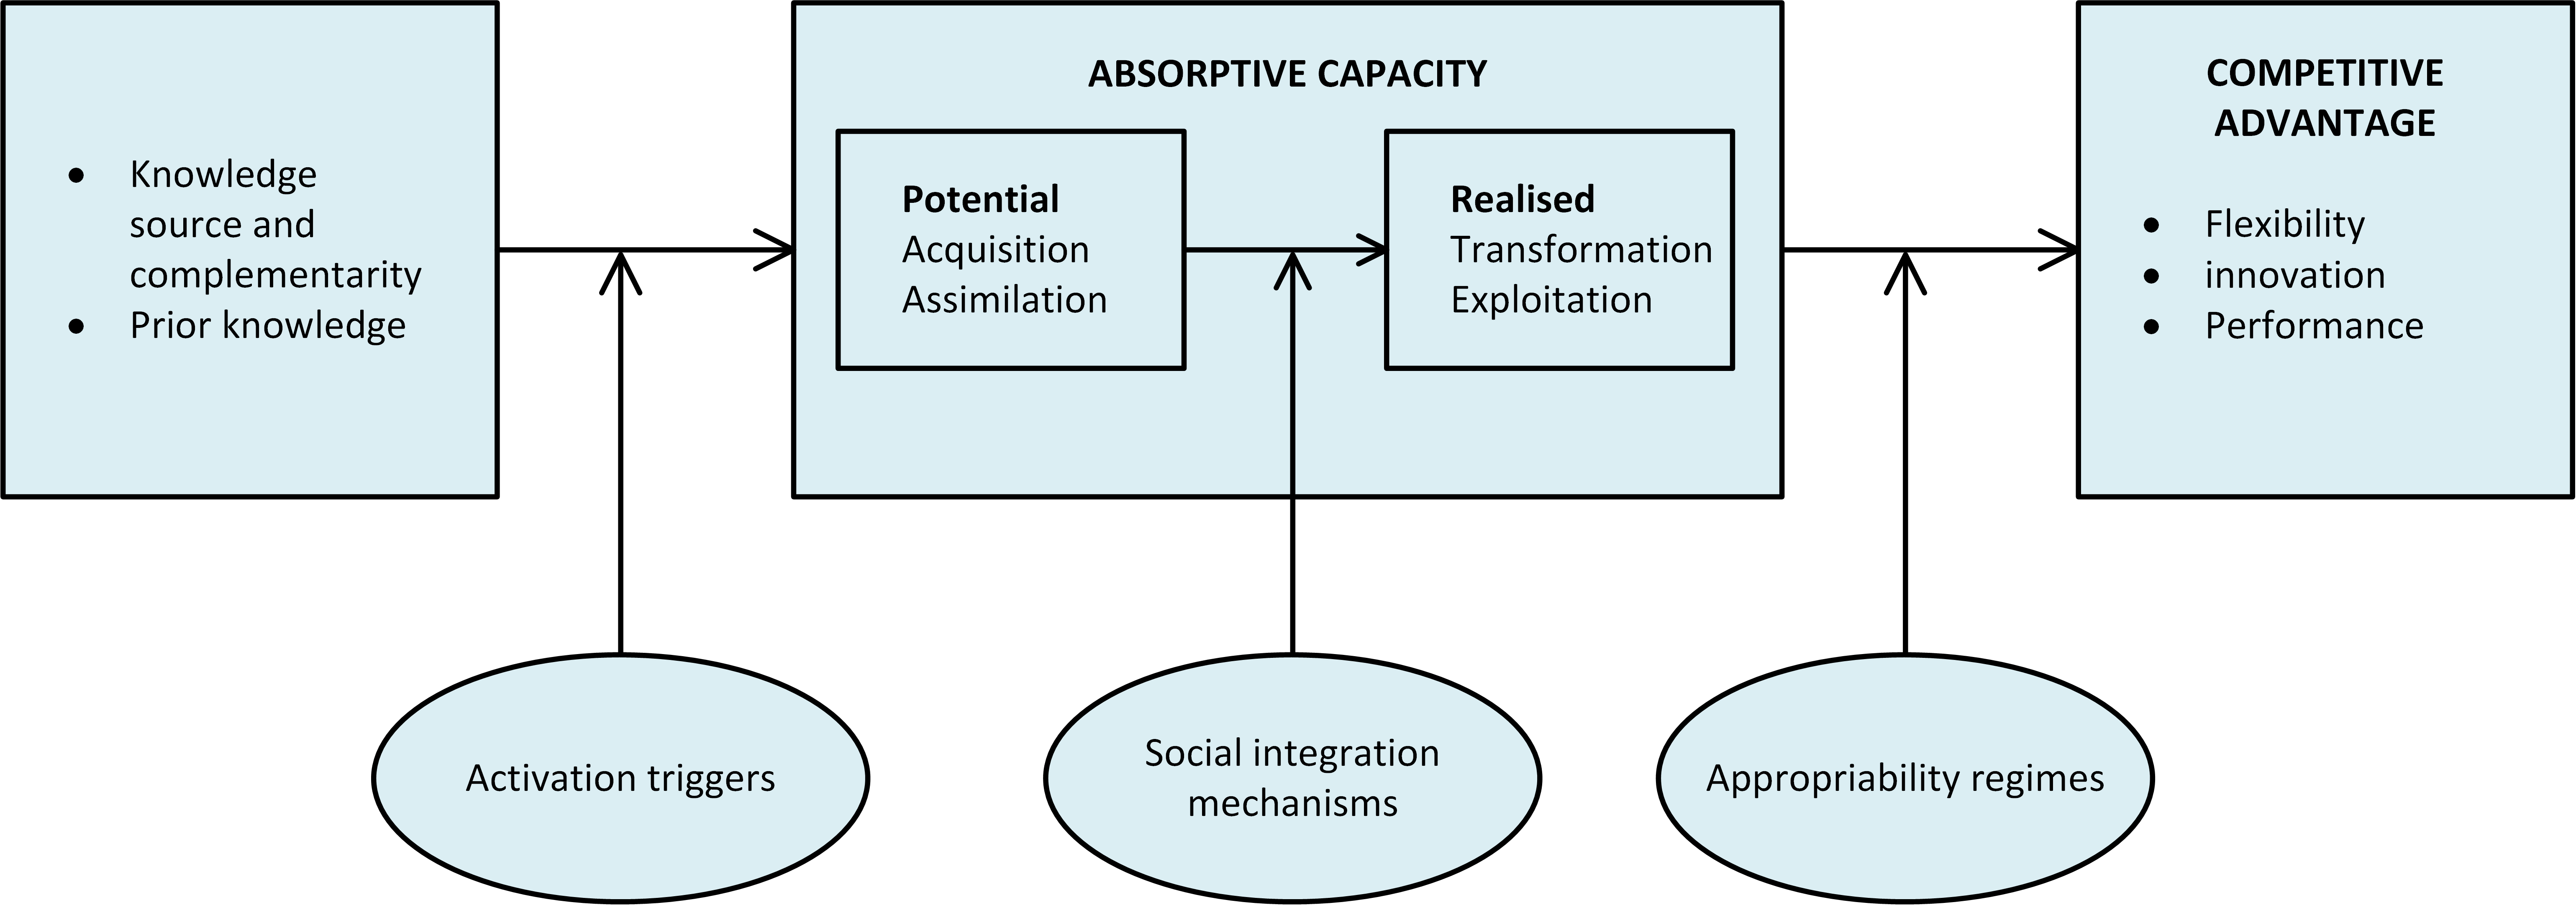
\includegraphics[width=0.9\linewidth]{Images/zahra_george}
	\caption{Process-based model of absorptive capacity \citep{zahra2002absorptive}.}
	\label{fig:zahrageorge}
\end{figure}


\citet{jansen2005managing} investigated the organisational antecedents of potential and realised absorptive capacity. They found that \enquote{coordination capabilities}, specifically brokerage, shared decision-making, and job rotation, enhance potential absorptive capacity, whereas \enquote{socialisation capabilities} that deal with connections to the organisational hierarchy and efforts to encourage social interaction increase realised absorptive capacity. In addition, they found that processes for embedding new knowledge into organisational routines, namely \enquote{systems capabilities}, contribute to realised absorptive capacity. Though the acquisition and assimilation of new knowledge can be formalised into organisational routines to some extent, this may not be the case with knowledge transformation, where formal routines are likely to restrict creativity \citep{jansen2005managing}. \medskip

According to \citet{lane2006reification}, process-oriented approaches to absorptive capacity highlight the importance of cognitive dimensions of learning. They considered absorptive capacity to be a firm's ability to apply externally held knowledge through three sequential learning processes. These include recognising and understanding potentially valuable new knowledge outside the firm through \enquote{exploratory learning}, assimilating valuable new knowledge via \enquote{transformative learning}, and using the assimilated knowledge to generate new knowledge and create commercial outputs through \enquote{exploitative learning}. \citet{lane2006reification} claimed that conceptualising absorptive capacity in terms of learning processes is a good starting point for developing a more comprehensive model of a firm’s absorptive capacity that includes both drivers and outcomes.\medskip

\citet{todorova2007absorptive} argued that \citet{zahra2002absorptive} discounted important insights of \citet{cohen1990absorptive} relating to learning and innovation. \citet{cohen1990absorptive} viewed the relationship between absorptive capacity and the level of prior-related knowledge as a positive feedback or learning loop where an increase in absorptive capacity improves the level of prior-related knowledge, which in turn further increases absorptive capacity. \citet{todorova2007absorptive} proposed that closer examination of feedback relationships should contribute to a better understanding of the dynamic nature of absorptive capacity. They also highlighted the importance of recognising the value of knowledge as a precursor to knowledge acquisition, which is often constrained by bounded rationality \citep{simon1972theories,cohen1990absorptive,ocasio1997towards}. Similar to \citet{cohen1990absorptive}, \citet{todorova2007absorptive} argued that recognising the value of knowledge is important, believing \citet{zahra2002absorptive} should not have dropped this aspect in their reconceptualisation of absorptive capacity. They also did not see the absorptive capacity processes working sequentially as suggested by \citet{zahra2002absorptive}. Instead, the different processes are more likely to interact and reinforce each other. This implies that the ratio of realised absorptive capacity to potential absorptive capacity is a poor measure of the efficiency of an organisation at leveraging absorbed knowledge. \medskip

\citet{todorova2007absorptive} described the contingent factors that they think are important to absorptive capacity. These include the mechanisms for achieving social integration, the strength or weakness of different appropriability regimes, and the nature of power-relations. Because absorptive capacity is something that emerges through social interaction, they argued that any conceptualisation of absorptive capacity should account for the mechanisms governing social interaction. \citet{cohen1990absorptive} claimed that a firm's willingness to invest in absorptive capacity is contingent on the strength of appropriability regimes. \citet{todorova2007absorptive} claimed that understanding appropriability regimes is a vital prerequisite to absorptive capacity and that firms do not want to leak valuable knowledge as quickly as they absorb it. Regarding power-relations, \citet{todorova2007absorptive} suggested that internal power relationships moderate the impact of assimilation or transformation on the application of new knowledge, while external power relationships moderate the relationship between absorptive capacity and competitive advantage. Figure \ref{fig:todorova} depicts \citet{todorova2007absorptive}'s conceptualisation of absorptive capacity. \medskip

\begin{figure}
	\centering
	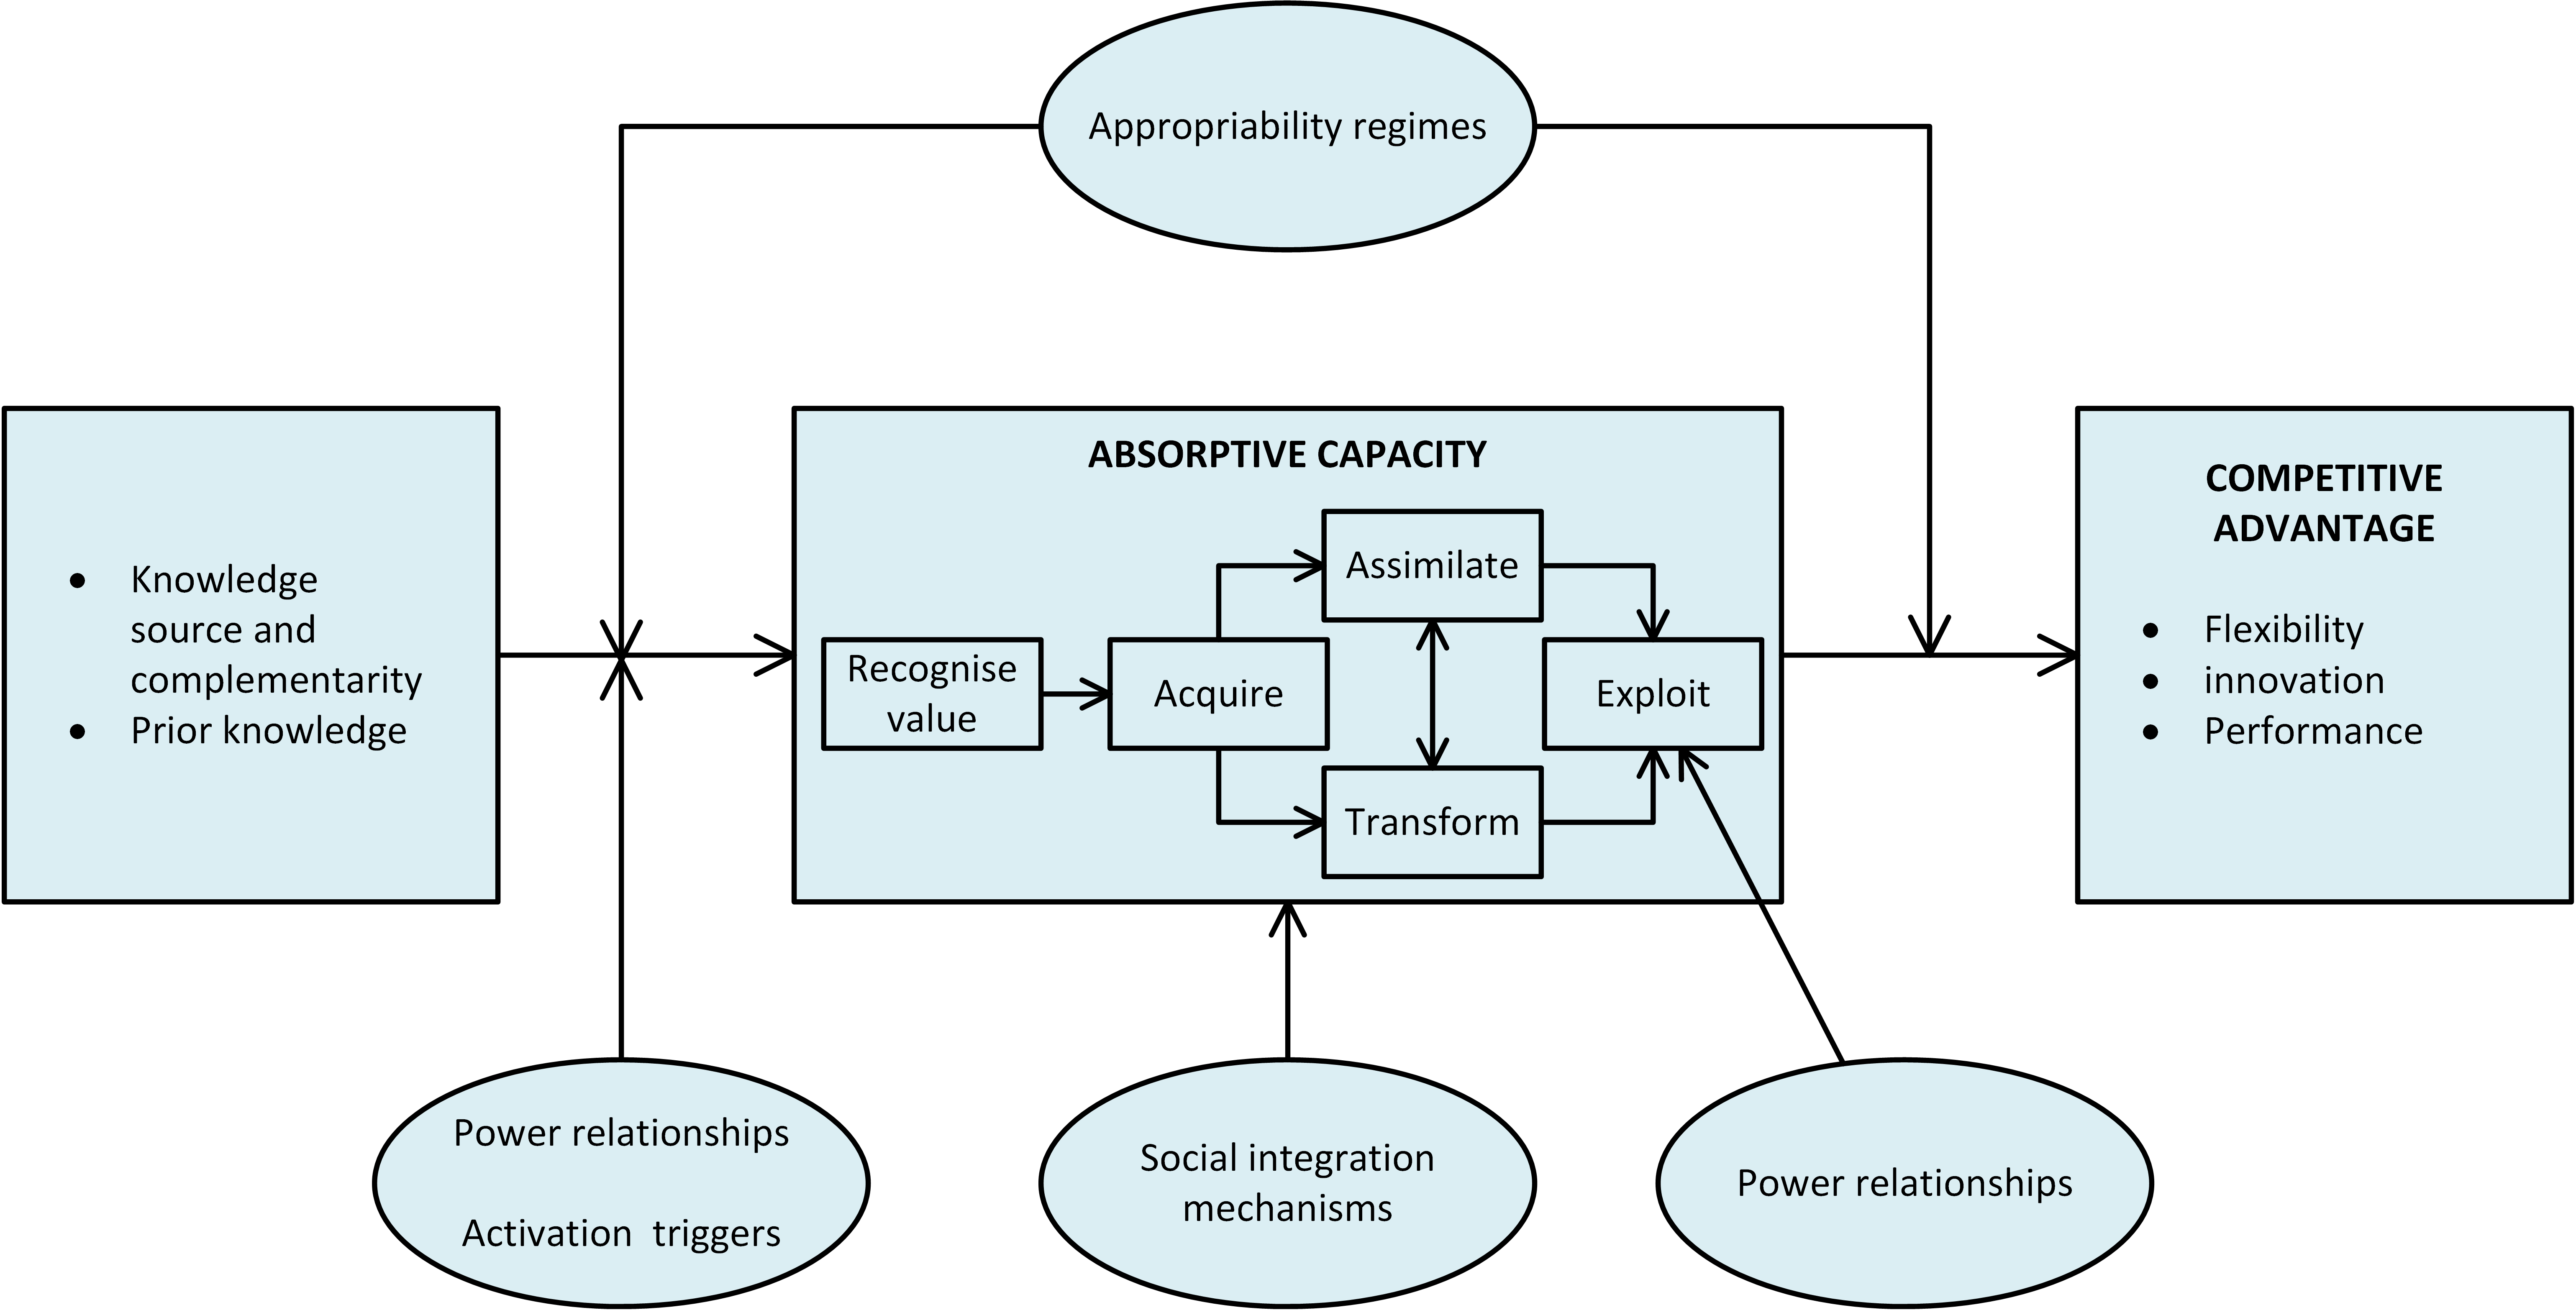
\includegraphics[width=0.9\linewidth]{Images/todorova}
	\caption{A refined model of absorptive capacity \citep{todorova2007absorptive}.}
	\label{fig:todorova}
\end{figure}

\citet{easterby2008absorptive} investigated the processes for acquiring, assimilating, transforming, and exploiting new knowledge in three cases and found that absorptive capacity is moderated by power-relations. They distinguished between power involving discrete political acts by self-interested actors, referred to as \enquote{episodic power}, and power which is diffused through social structures, referred to as \enquote{systemic power}. They observed that external access to knowledge is affected by episodic power, while the diffusion of knowledge within a firm depends mainly on systemic power. \medskip

Furthermore, \citet{easterby2008absorptive} argued that past studies on absorptive capacity have taken boundaries for granted. They claimed that it is important to understand the nature of boundaries and how these affect absorptive capacity processes. Boundaries are difficult to define, vary considerably in permeability, and can change significantly over time. Per \citet{easterby2008absorptive}, the permeability of boundaries determines the ease knowledge can be transferred. They refer to \enquote{syntactic}, \enquote{semantic} and \enquote{pragmatic} approaches to knowledge transfer \citep{carlile2004transferring}. The syntactic approach involves the transfer of data through information technology, the semantic approach focuses on the translation of language and creation of shared meanings, and the pragmatic approach focuses on transforming knowledge through political efforts and negotiation of practices. \citet{easterby2008absorptive} noted a progression from syntactic to pragmatic modes as organisations increase their absorptive capacity. They considered power and boundaries as central features of a process view of absorptive capacity. \medskip

\citet{volberda2010perspective} presented an integrative framework of absorptive capacity that identifies the organisational antecedents, process dimensions, and outcomes of absorptive capacity (Figure \ref{fig:volberdaintegrativemodel}). The framework also considers contextual or environmental factors affecting absorptive capacity and highlights significant gaps in the understanding of absorptive capacity. These include the need to achieve better insight into the processes and routines that generate absorptive capacity and how these drive individual and organisational actions that lead to innovations and competitive advantage \citep{volberda2010perspective}. \medskip

\begin{figure}
	\centering
	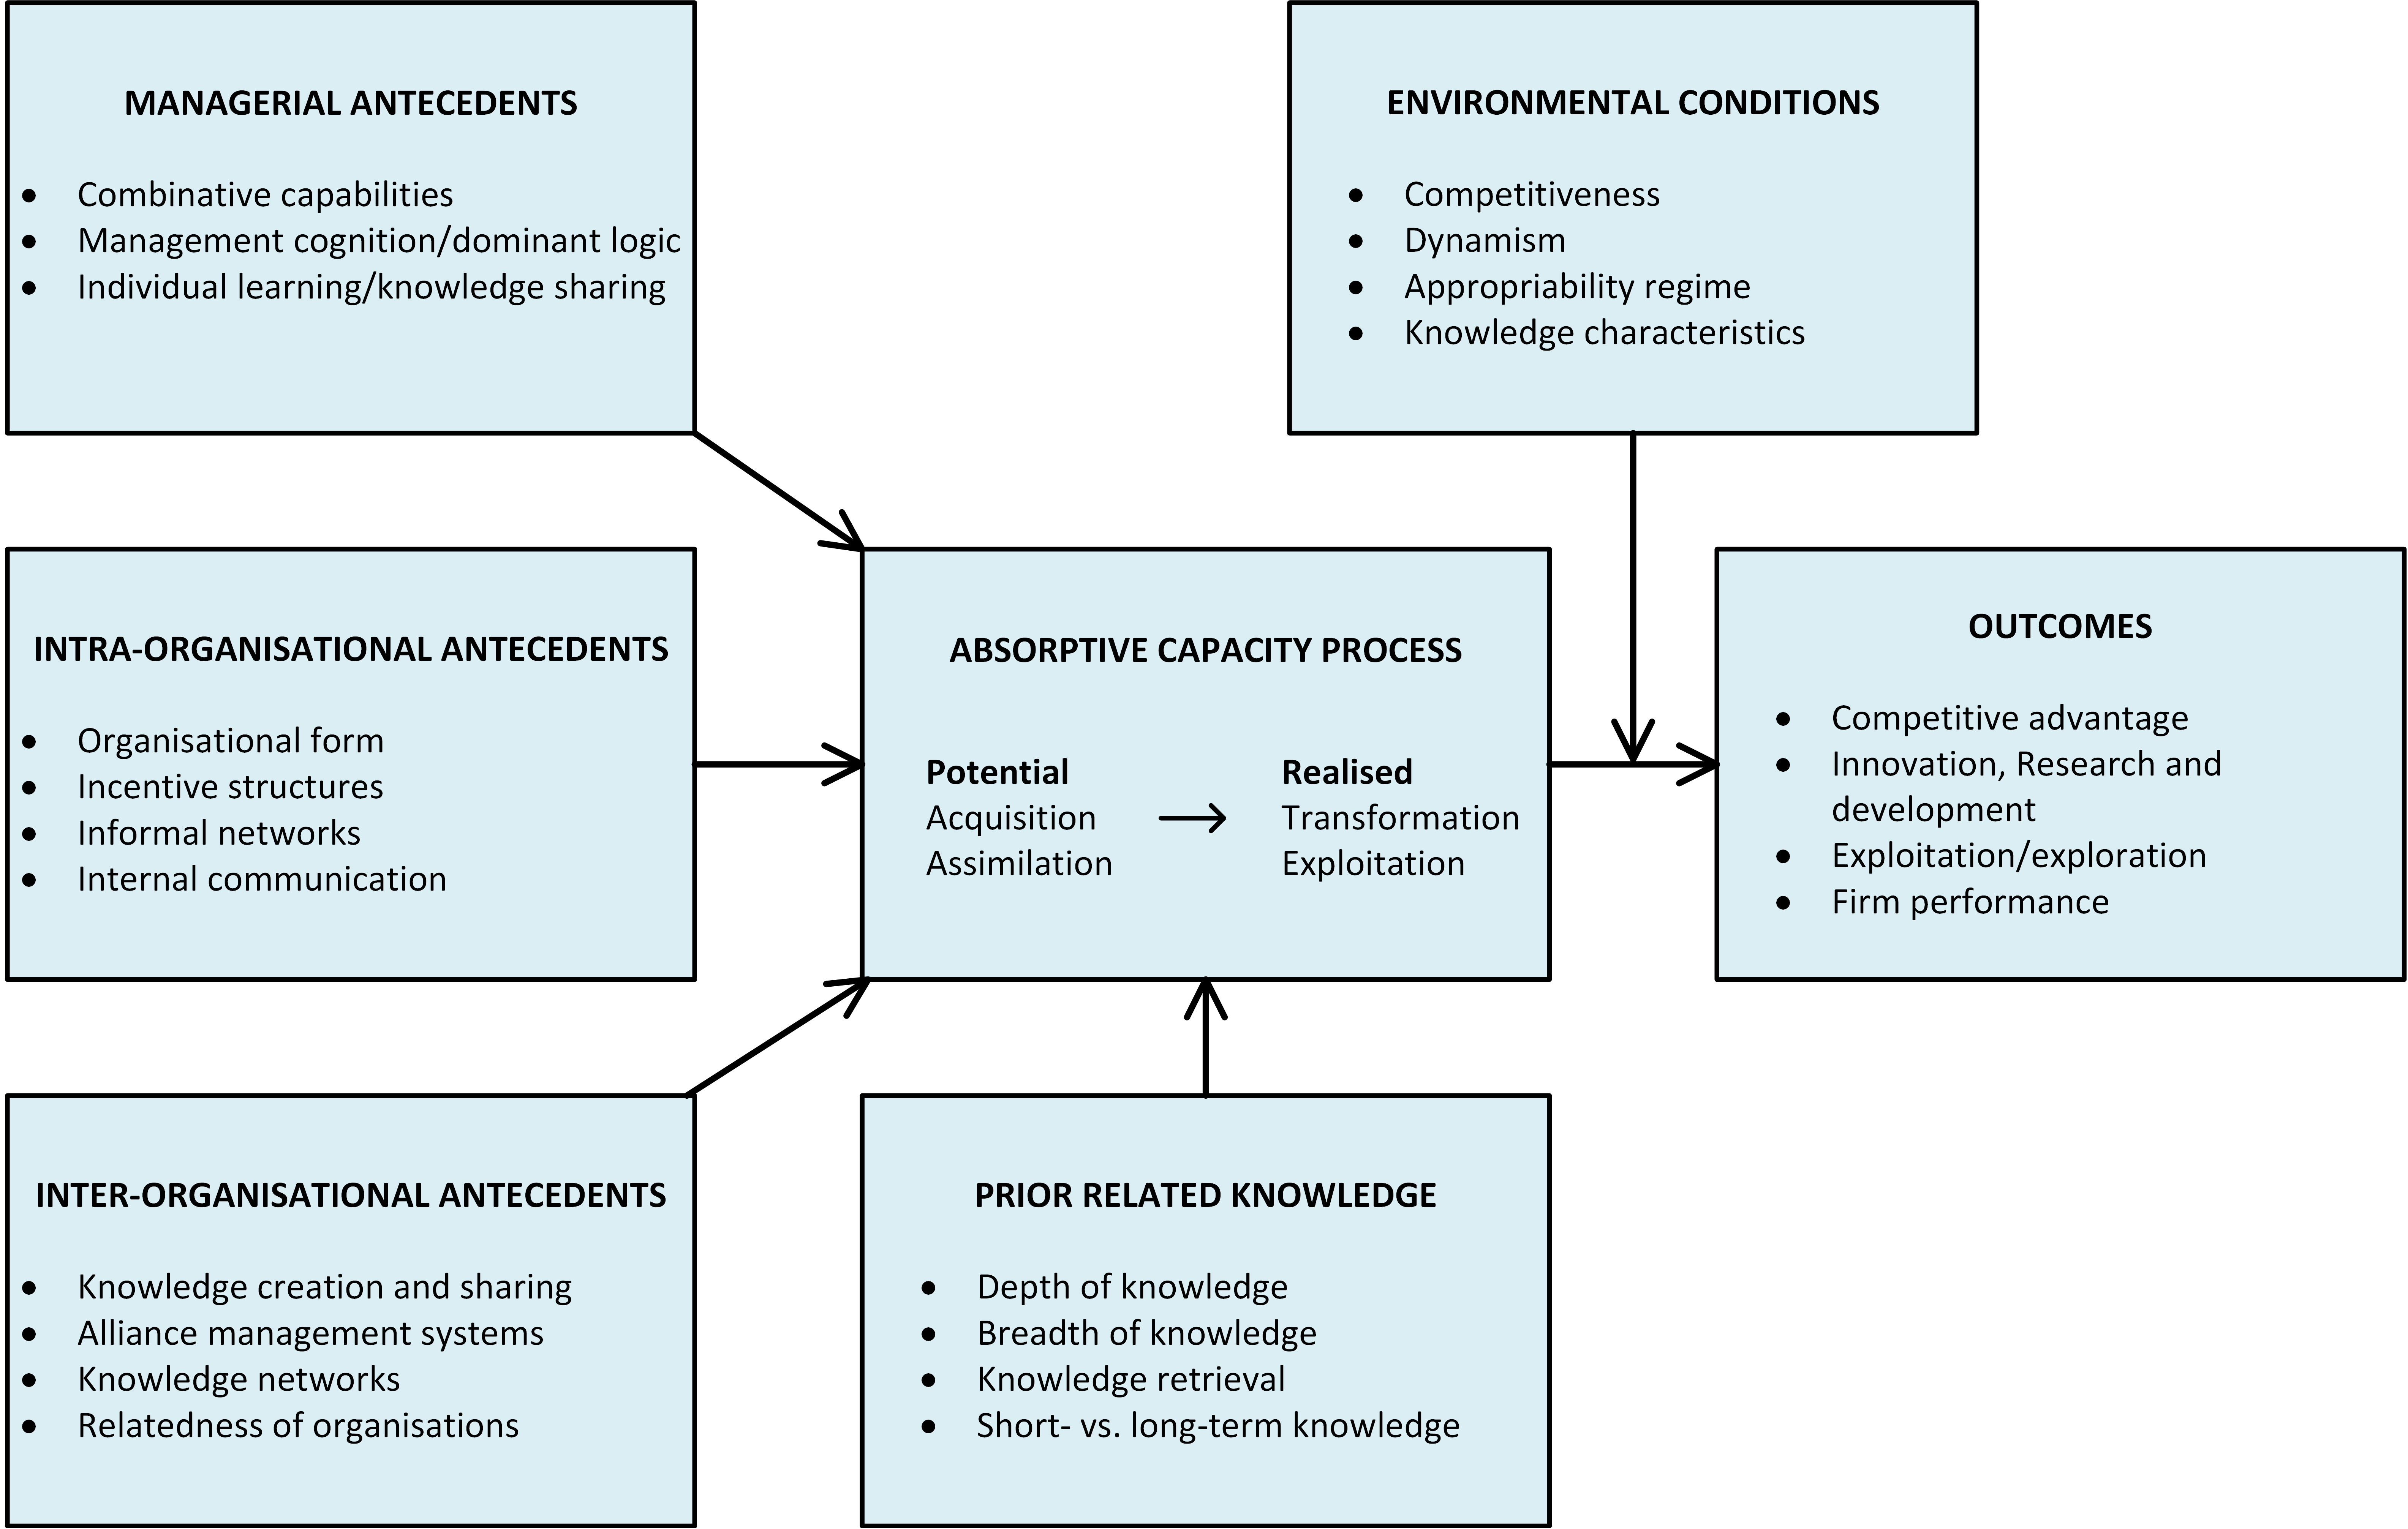
\includegraphics[width=1.0\linewidth]{Images/Volberda_Integrative_Model}
	\caption{An integrative framework of absorptive capacity \citep{volberda2010perspective}.}
	\label{fig:volberdaintegrativemodel}
\end{figure}

The routine-based model of absorptive capacity developed by \citet{lewin2011microfoundations} addresses some of the gaps highlighted by \citet{volberda2010perspective}. \citet{lewin2011microfoundations} suggested that routines are the building blocks of organisational capabilities, which take the form of rules, procedures, norms, or practices unique to each firm. Routines embody both explicit and tacit knowledge and are assumed to evolve through organisational learning processes. \citet{lewin2011microfoundations} distinguished between internal routines that support the creation, transformation, application and assimilation of knowledge internally and external routines that allow the acquisition, assimilation, transformation and exploitation of new external knowledge. They argued that uncovering the configuration of routines that constitute the absorptive capacity of a firm and their expression in everyday practices is central to understanding the mediating role of absorptive capacity in innovation. \medskip

\citet{marabelli2014knowing} suggested that a firm's absorptive capacity should be interpreted in terms of the \enquote{epistemology of possession} and the \enquote{epistemology of practice}. The epistemology of possession treats knowledge as something people possess and can be transferred. It emphasises explicit over tacit knowledge and knowledge held by individuals over that possessed by groups. This epistemology cannot account for knowledge found in individual and group practice \citep{cook1999bridging}. The epistemology of practice, on the other hand, assumes that knowledge is unpredictable and dynamic in nature and constituted in and through practice \citep{marabelli2014knowing}. Knowledge located in individual or group practice is not transferable and requires mediators to translate and recreate knowledge through practices in other settings \citep{marabelli2012knowledge}. The epistemology of practice treats absorptive capacity as a capability that emerges when knowledge is used in practice, and this epistemology can be used to explain how knowledge moves between the different phases of absorptive capacity \citep{marabelli2014knowing}. \medskip

The epistemology of practice can also help explain power-relations. \citet{marabelli2014knowing} claimed that \citet{todorova2007absorptive} have too narrow a perspective of power, treating it as something people possess, and discounting the politics of power-relations or the multiple dimensions of power. \citet{marabelli2014knowing} argued that a practice-based perspective provides a more nuanced perspective of power and how it shapes absorptive capacity. They referred to \enquote{prohibitive power} and \enquote{productive power} (also referred to as \enquote{power-over} and \enquote{power-to}, respectively). Prohibitive power focuses on the capacity of organisational actors to control resources and achieve objectives at the expense of others. Productive power, on the other hand, focuses on empowering (or dis-empowering) actors to change the ways things are done in practice. \medskip

\citet{marabelli2014knowing} adapted the integrative framework of absorptive capacity described by \citet{volberda2010perspective}. They differentiated between the elements considered relevant to the possession perspective and elements aligned with the practice perspective. \citet{marabelli2014knowing} showed how important it is to consider not only the acknowledged structural and cognitive elements that affect absorptive capacity, but also the ways in which these are enacted in practice. \citet{marabelli2014knowing} argued that innovation does not moving smoothly from the acquisition of new ideas through the development of these ideas during assimilation and transformation to the final application as an innovation. Rather, these processes are more likely to operate concurrently, reflecting the messy unfolding of innovation in practice, which is a phenomenon that is continuously influenced by power. \citet{marabelli2014knowing} claimed that the interplay between both types of power has implications regarding how absorptive capacity emerges. \medskip

A recent article by \citet {lichtenthaler2016absorptive} suggested past studies have overlooked the downsides of building absorptive capacity. These include challenges around capturing value, overemphasis regarding prior-related knowledge, and inter-dependencies between internal processes. The challenges around capturing value relate to the capabilities needed to manage the increasingly complex knowledge and the rising cost of capability development. \citet{lichtenthaler2016absorptive} claimed that knowledge is often tacit, context-specific, and perishable in nature. According to him, firms struggle to capture value from tacit knowledge and prior related knowledge may be of limited use when it comes to adapting and transforming knowledge for use in new contexts. Moreover, some firms may not benefit from externally sourced knowledge because it may decay over time. In addition, \citet{lichtenthaler2016absorptive} mentioned the multilevel nature of absorptive capacity. While interactions between different levels can enrich absorptive capacity, this increases its complexity, possibly leading to less favourable outcomes. Absorptive capacity also varies considerably across organisations. \citet{lichtenthaler2016absorptive} claimed that relative differences in absorptive capacity can make it more difficult to transfer knowledge across organisational boundaries. Even firms with high levels of absorptive capacity may still encounter major managerial challenges in acquiring knowledge from a partner with different organisational characteristics. \citet{lichtenthaler2016absorptive} argued that the development and maintenance of absorptive capacity requires money and resources. He stated that determining the cost-benefit of absorptive capacity is difficult, given its complexity. \medskip

\begin{figure}
	\centering
	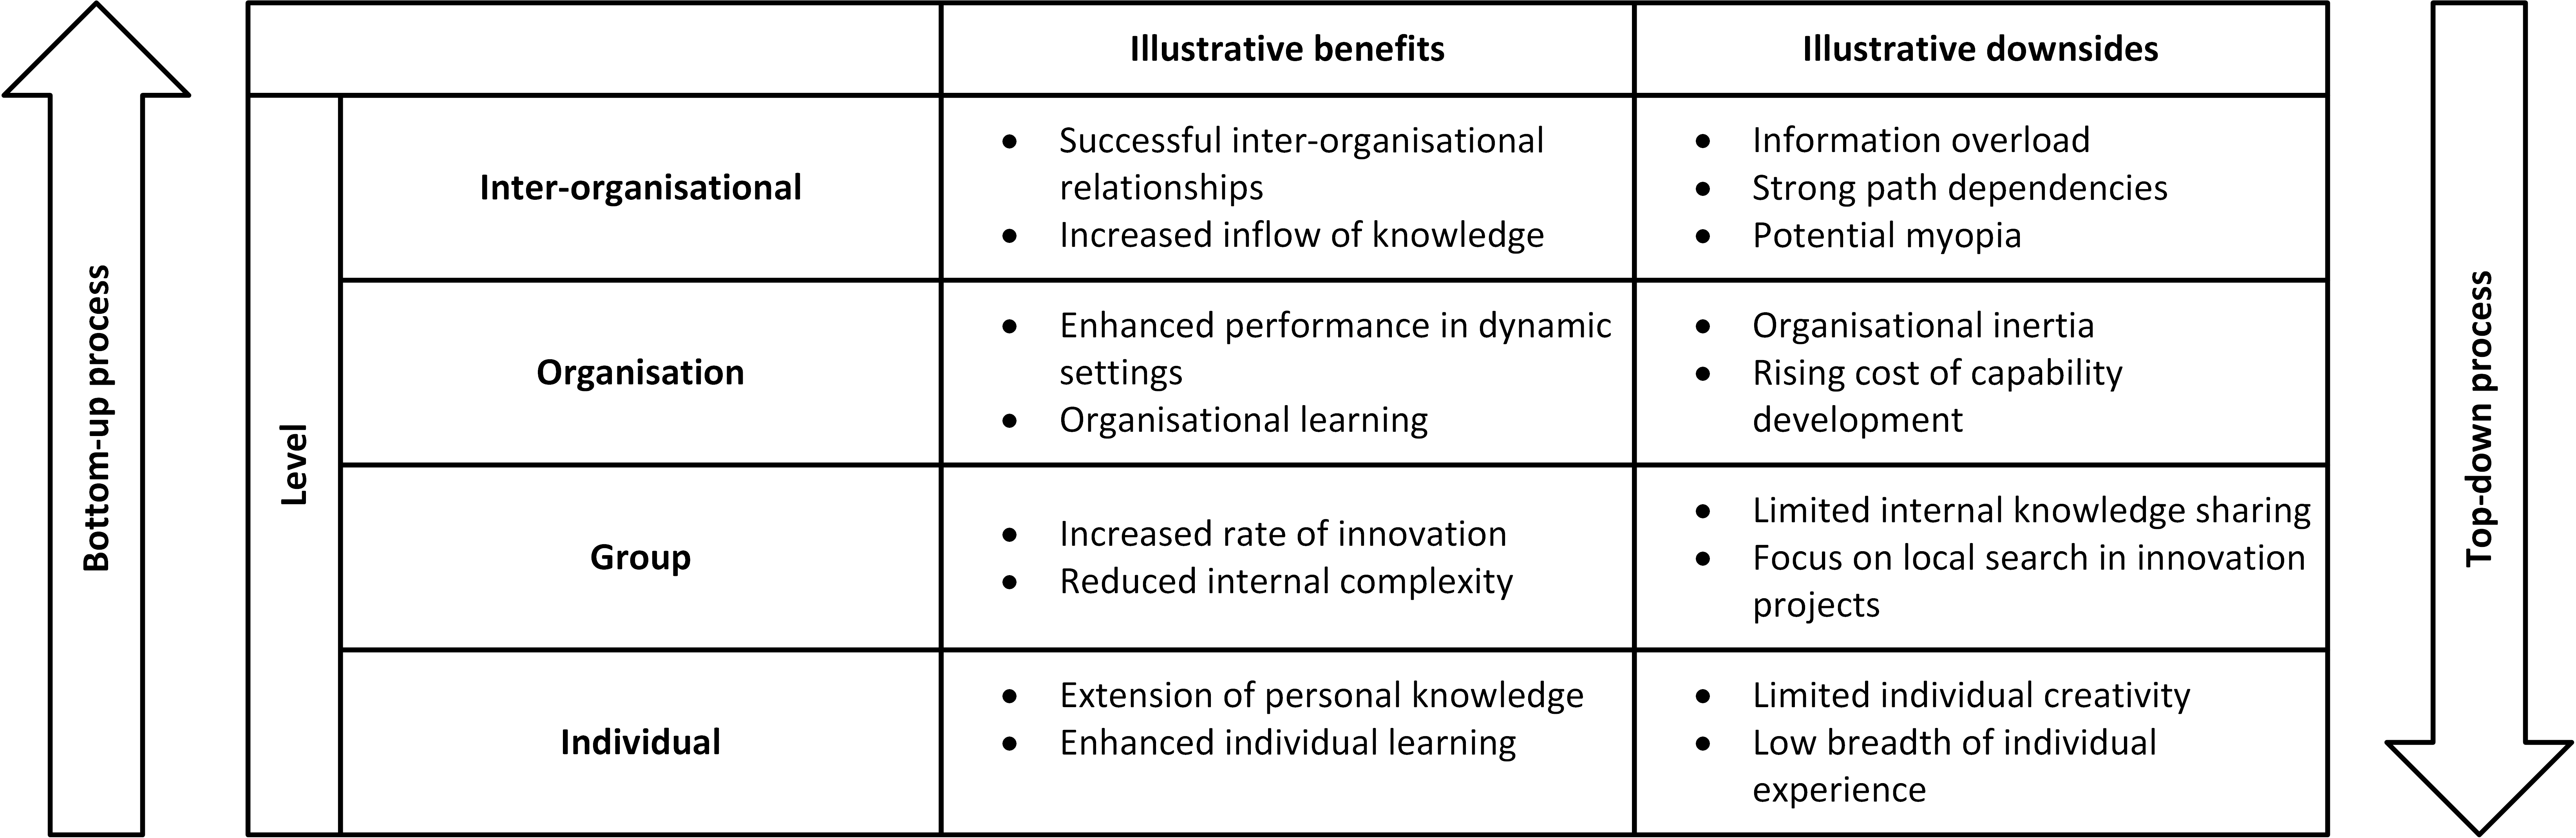
\includegraphics[width=0.9\linewidth]{Images/updownsides}
	\caption{Benefits and downsides of absorptive capacity at multiple levels \citep{lichtenthaler2016absorptive}.}
	\label{fig:updownsides}
\end{figure}

\citet{lichtenthaler2016absorptive} also claimed that over-reliance on prior related knowledge may result in a firm completely ignoring new knowledge. He stated that there needs to be a trade-off between having prior knowledge for building and maintaining absorptive capacity and being able to find additional novelty in external knowledge. \citet{lichtenthaler2016absorptive} also claimed that firms need to find the right balance between internal knowledge development and external knowledge acquisition. When firms focus on external knowledge acquisition, they may forego the benefits from sharing internal knowledge. This may be particularly detrimental in large and diversified firms with diverse knowledge bases. \medskip 

Absorptive capacity is a complex multidimensional and somewhat abstract construct that is difficult to quantify or assess in practice. Theoretically, it is located between the fields of dynamic capability, organisational learning, and knowledge management \citep{easterby2008absorptive}. Most scholars have agreed that absorptive capacity is a dynamic capability that allows firms to cope with rapidly changing external environments, capture value from externally sourced knowledge, and improve alliance performance \citep{omidvar2013revisiting}. Though absorptive capacity can be treated as a form of organisational learning \citep{cohen1989innovation,easterby2008absorptive,sun2010examination}, it cannot be reduced to the actions of cognising subjects \citep{omidvar2013revisiting,turner2013absorptive,marabelli2014knowing}. \medskip

\section{Open innovation context}

\citet{vanhaverbeke2007connecting} suggested that insights from the best practices in open innovation can enrich the concept of absorptive capacity. They claimed that firms need absorptive capacity to engage in open innovation. Moreover, they suggested that combining the resource-based view \citep{wernerfelt1984resource} and relational perspective of the firm \citep{dyer1998relational} leads to a better understanding of absorptive capacity. \citet{vanhaverbeke2007connecting} also argued that open innovation is much more explicit regarding the different organisational practices for external-knowledge sourcing. They claimed that relating absorptive capacity to open innovation opens new avenues to re-conceptualise absorptive capacity into a more grounded concept that is valuable for managerial practice. \medskip

\citet{lichtenthaler2009capability} claimed that the different conceptualisations of absorptive capacity focus too much on external knowledge and do not address other important knowledge processes found in open innovation. They presented a conceptual framework that includes six knowledge management capacities that address knowledge exploration, retention, and application inside and outside the firm. Figure \ref{fig:oiaccapabilityframework} illustrates how these capacities contribute to intra-firm and inter-firm knowledge processes. \citet{lichtenthaler2009capability} described \enquote{inventive capacity} as a firm’s ability to create new knowledge inside the firm. They treated \enquote{absorptive capacity} simply as a firm’s ability to explore external knowledge. Because knowledge transformation involves the reactivation of retained knowledge, \citet{lichtenthaler2009capability} referred to the ability of a firm to retain knowledge over time as \enquote{transformative capacity}. They treated \enquote{connective capacity} as the ability of a firm to retain knowledge in inter-organisational relationships and \enquote{innovative capacity} as the ability for a firm to internally apply knowledge. \enquote{Desorptive capacity} refers to a firm’s ability to apply knowledge externally. \citet{lichtenthaler2009absorptive} claimed their framework complements absorptive capacity because it contributes to a better understanding of dynamic capabilities required for managing knowledge flows in open innovation. \medskip

\begin{figure}
	\centering
	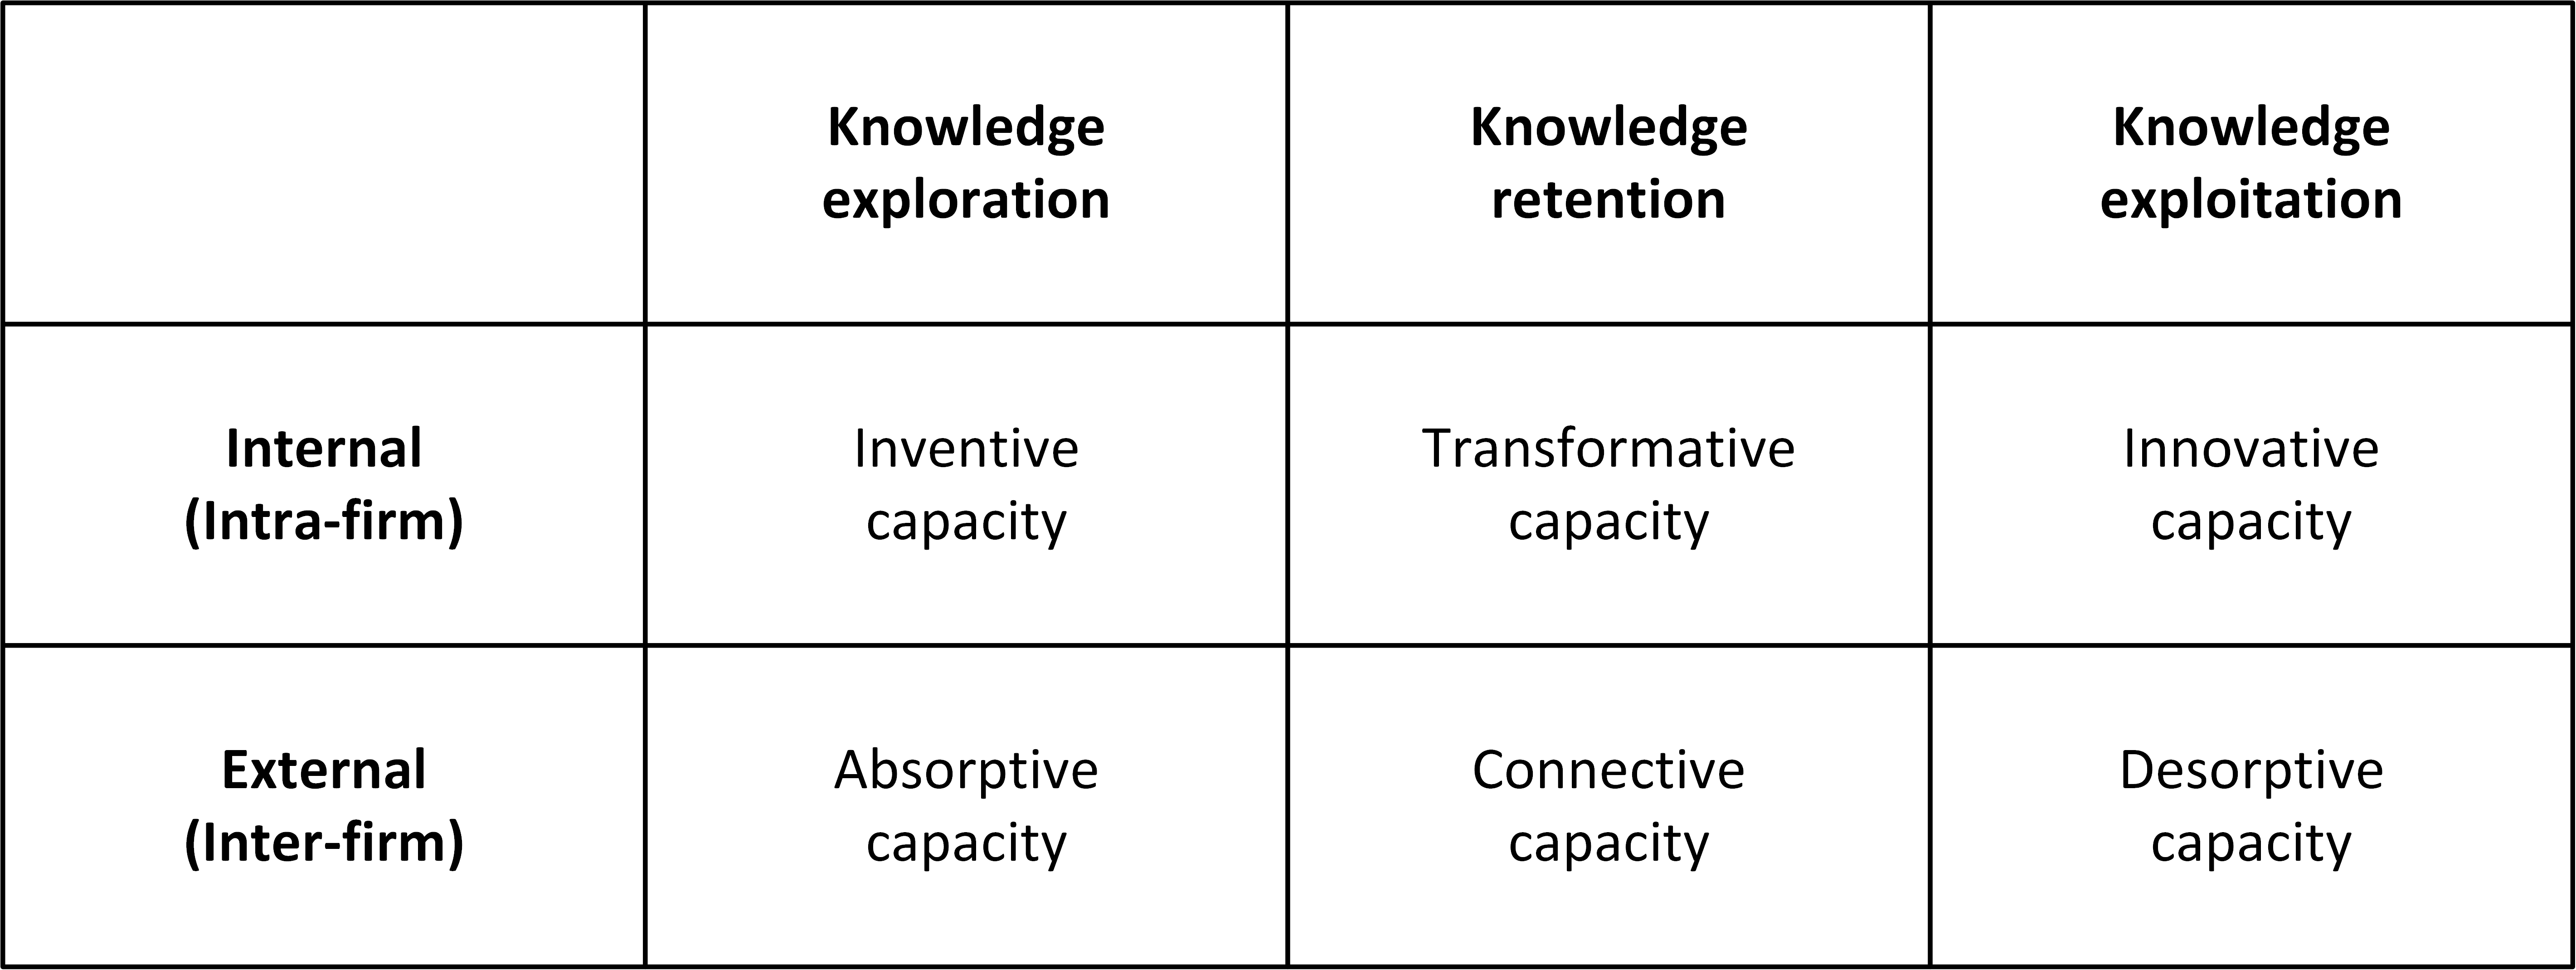
\includegraphics[width=0.7\linewidth]{Images/oi_ac_capability_framework}
	\caption[Capability framework for open innovation]{Capability framework for open innovation \citep{lichtenthaler2009capability}}
	\label{fig:oiaccapabilityframework}
\end{figure}

Using similar reasoning to \citet{lichtenthaler2009absorptive}, \citet{robertson2012managing} argued that firms pursuing open innovation need specific innovative capacities that extend beyond those needed for knowledge management \citep[e.g.][]{zahra2002absorptive,todorova2007absorptive,lichtenthaler2009capability}. These include \enquote{accessive capacity} to collect, sort and analyse knowledge sourced internally and externally; \enquote{adaptive capacity} to ensure new technology can be re-purposed to suit the firm's needs; \enquote{integrative capacity} to allow new or adapted technology to be integrated into existing processes or systems; and an \enquote{innovative management capacity} to serve as a higher-order dynamic capability to control and coordinate a firm's innovative capacities. \citet{robertson2012managing} suggested that these innovative capacities provide a better understanding of knowledge application processes. \medskip

Key mechanisms underpinning open innovation were tested by \citet{ahn2016beyond} using a hierarchical model encompassing organisational openness, innovative capacities and firm performance. They argued that a firm's performance depends on the extent to which innovative capacities are moderated by its degree of openness, which is defined as the \enquote{propensity of a firm for implementing open innovation}. \citet{ahn2016beyond} viewed \enquote{search capacity}, \enquote{integrative capacity}, \enquote{knowledge management capacity}, and \enquote{desorptive capacity} to constitute a firm's innovative capacities. They treated absorptive capacity as a higher-order capability that encompasses search and integrative capacity. Results from their survey of Korean firms show that apart from knowledge management, innovative capacities directly influence firm performance. Furthermore, they found that knowledge management capacity indirectly influences firm performance via desorptive capacity. \citet{ahn2016beyond} claimed that the strong relationship between search and integrative capacities and firm performance confirms the importance of absorptive capacity in open innovation. They also found that outbound open innovation plays an important role in improving firm performance. \medskip

\citet{hughes2010knowledge} examined the capabilities needed for open innovation and how these relate to absorptive capacity in a case study involving a multinational pharmaceutical company. They found that experimental learning and sharing of best practices helps build capabilities for open innovation. This involves exposing customers to research and development processes, forming collaborative partnerships with customers and extending existing research and development collaboration networks. \citet{hughes2010knowledge} claimed that the concept of absorptive capacity needed to be refined to address bi-directional knowledge flows in open innovation. \medskip

\citet{xia2016unpacking} explored the link between internal absorptive capacity and external relationships in open innovation. Building on ideas promoted by \citet{march1991exploration} and \cite{rothaermel2004exploration}, they distinguished between exploratory relationships that aim to discover something new, and relationships that aim to join existing competencies across organisational boundaries to gain synergistic benefits. Results from a survey of 349 pharmaceutical firms in Europe and the United States suggest that realised absorptive capacity plays an important role in the growth of firms. \cite{xia2016unpacking} found that the engagement in exploratory relationships depends strongly on the continuity of internal research and development to properly assimilate new external knowledge. Participation in relationships that aim to join existing competencies depends largely on the realised absorptive capacity of partner firms. \citet{xia2016unpacking} supported calls to investigate more deeply knowledge application processes in open innovation \citep[e.g.][]{lichtenthaler2009absorptive,lichtenthaler2010technology,robertson2012managing} investigated the capabilities needed for managing bi-directional knowledge flows \citep[e.g.][]{gassmann2010future,hughes2010knowledge}. \medskip

The attention-based view assumes that a firm's behaviour depends on how it channels the attention of its decision-makers, and firms tend to direct their limited resources to issues that attract their short-run attention, often to the detriment of their long-run performance \citep{ocasio1997towards}. \citet{kim2016balancing} used the attention-based view to help explain the development of absorptive capacity in open and closed inbound innovation. They argued that innovation is about overcoming attentional constraints by redirecting attention to otherwise ignored knowledge sources in different technology domains or other organisations, while overcoming resource constraints is through the redeployment or acquisition of resources. Innovation is more likely to occur when a firm allocates attention to the recognition, assimilation, and application of new knowledge inside and outside the firm. \citet{kim2016balancing} suggested that open and closed inbound innovation require different types of absorptive capacity, namely \enquote{inward-looking absorptive capacity} for closed inbound innovation, and \enquote{outward-looking absorptive capacity} for open-inbound innovation. They claimed that firms should practice switching their attention between open and closed inbound innovation repeatedly to develop their absorptive capacity. This enables firms to find the optimum balance between potential and realised absorptive capacity and between inward-looking and outward-looking absorptive capacity. Firms that obtain the correct balance find it easier to cross technological and organisational boundaries, leading to enhanced innovative performance. \medskip

Because of open innovation, absorptive capacity is becoming a more grounded concept of practical value \citep{vanhaverbeke2007connecting,lichtenthaler2009capability}. Much of the attention in absorptive capacity research has been on knowledge application inside the firm. While there is a clear connection between absorptive capacity and inbound open innovation, this is not the case with outbound or coupled open innovation, which is about knowledge application outside the firm. Open innovation focuses on the distinction between potential and realised absorptive capacity. Recent studies suggest that realised absorptive capacity is important for outbound open innovation \citep[e.g.][]{kim2016balancing,xia2016unpacking}. The concept of absorptive capacity has increasingly been treated as one of many capacities needed for open innovation \citep[e.g.][]{lichtenthaler2009capability,lichtenthaler2010technology,robertson2012managing,ahn2016beyond}. There is a good chance that absorptive capacity will be treated more narrowly in the future as it becomes more disaggregated \citep[viz.][]{lichtenthaler2009capability}. \medskip

\section{Measuring absorptive capacity}

Different conceptualisations have frustrated efforts to develop an agreed measurement of absorptive capacity \citep{duchek2013capturing}. Early approaches used either input-oriented measures, such as investment in research and development \citep[e.g.][]{rocha1999inter,stock2001absorptive,becker2000technological} or number of employees with post-graduate degrees \citep[e.g.][]{veugelers1997internal,gao2008knowledge}, or output-oriented measures, such as the number of publications and patents \citep[e.g.][]{cockburn1998absorptive,george2001effects}, as proxy measurements of absorptive capacity. Later approaches have either employed perceptive instruments to measure components of absorptive capacity \citep[e.g.][]{szulanski1996exploring,jansen2005managing,nieto2005absorptive,flatten2011measure} or used case studies to expose key processes influencing absorptive capacity \citep[e.g.][]{kim1998crisis,van1999coevolution,jones2001expanding,jones2006developing,easterby2008absorptive}. \medskip

Quantitative measures fail to capture the complex and dynamic nature of absorptive capacity \citep{easterby2008absorptive,duchek2013capturing}. Though qualitative studies have yielded new perspectives on absorptive capacity, these tend to address knowledge absorption practices in specific settings and pay scant attention to the constituent elements of absorptive capacity \citep{duchek2013capturing}. As mentioned earlier, recent studies point to a practice-based approach as most appropriate for identifying the routines and practices that build absorptive capacity \citep[e.g.][]{duchek2013capturing,omidvar2013revisiting,marabelli2012knowledge,marabelli2014knowing}. \citet{duchek2013capturing} claimed that qualitative methods, such as ethnography and narrative inquiry, allow one to study practices in real-world situations. These methods not only enable a researcher to study the dynamic nature of practices, but also gain insight into the complex social, cultural, and political systems that organisations represent \citep{duchek2013capturing}. \medskip

\section{Sticky knowledge}

Past studies of absorptive capacity have emphasised the importance of prior knowledge possessed by individuals and groups. Most of these studies have treated knowledge as explicit, something that can be acquired, stored, processed, and retrieved \citep{omidvar2013revisiting,marabelli2014knowing}. In reality, much of the prior knowledge possessed by individuals and groups is tacit, held either in people's minds or in the form of unwritten rules or practices that guide the collective action of groups \citep{mowery1996strategic,leonard1998role,burt2007secondhand,goksel2016can,lichtenthaler2016absorptive}. \citet{nelson1982evolutionary} suggested that organisations maintain their structure and coherency through tacit knowledge embedded in organisational routines that no single person completely understands. \medskip

Explicit and tacit knowledge should not be treated as a dichotomy, but rather as a spectrum with the two knowledge types at each extreme \citep{polanyi1967tacit,inkpen1998knowledge,cavusgil2003tacit}. At one extreme, it is almost completely tacit, that is knowledge held in peoples' minds and bodies. At the other extreme, knowledge is almost completely explicit, existing in codified or structured form and accessible to other people \citep{leonard1998role}. The knowledge resource available to a firm has been described as an iceberg. Explicit knowledge is the visible top of the iceberg. This part of the knowledge resource is easy to recognise and access. Beneath the surface of conscious thought is the hidden bulk of the iceberg, symbolising tacit knowledge resources derived from a lifetime of experience, practice, perception and learning \citep{spender1996making,haldin2000difficulties,mcadam2007exploring,rebernik2007fostering}. Tacit knowledge tends to be associated with terms such as \enquote{intuition}, \enquote{skill}, \enquote{know-how}, and \enquote{expertise} used to describe knowledge that refers to an ability to perform work \citep{mcadam2007exploring}. \citet{nielsen2002concept} conceptualised tacit knowledge in three different ways, namely tacit knowledge as a tradition, as an inexpressible dimension of practice, and as a form of intelligence. \medskip

Individual-based tacit knowledge is shared through social relations and communication, whereas group-based tacit knowledge is produced during group activities and is stored in shared memory, behaviours, automatic responses, and cognitive schemata \citep{goksel2016can}. A large amount of knowledge remains tacit for various reasons. One reason is that individuals may be reluctant to surrender any advantages their tacit knowledge or know-how affords them. Another reason is that people are either unaware of the tacit dimension of their knowledge or unable to express what they know \citep{leonard1998role,eraut2000non}. \medskip

Tacit knowledge is considered critical for innovation as it guides the thought processes that produce novel ideas \citep{leonard1998role,amar2008descriptive}. Because it is largely invisible, tacit knowledge is a tremendous source of competitive advantage \citep{nelson1982evolutionary,barney1991firm,grant1996toward,smith2001role,chilton2007dimensions,lu2015job}. The most common application of tacit knowledge is problem-solving. For instance, people with expertise from experience not only are able to recognise the situation in which they find themselves in, but also know which actions might be appropriate for dealing with it \citep{simon1971human,leonard1998role}. Tacit knowledge can also be used to reformulate problems by viewing these differently in intuitive ways. Intuition can also help predict or anticipate outcomes \citep{leonard1998role}.\medskip

Since tacit knowledge is unavailable for conscious inspection, it can only be assessed using indirect approaches \citep{chilton2007dimensions}. \citet{zander1995knowledge} characterised a firm's knowledge in terms of \enquote{codifiability}, \enquote{teachability}, \enquote{complexity}, \enquote{system dependence} and \enquote{product observability}. These five constructs measure the extent to which knowledge can be easily communicated and understood. Codifiability describes the extent to which knowledge can be declared and encoded. Teachability refers to the extent workers can be taught the knowledge required to do their jobs. Complexity refers to the inherent variations in combining different kinds of knowledge, while system dependence refers to the extent a capability is dependent on other experienced people for its production. Product observability refers to the degree knowledge can be operationalised by others \citep{winter1987knowledge,zander1995knowledge}. \citet{cavusgil2003tacit} studied how firms acquire tacit knowledge from collaboration partners and the extent to which tacit knowledge transfer affects innovation capability. They measured the extent of tacit knowledge transfer using \enquote{codifiability}, \enquote{complexity}, and \enquote{observability}. Their results indicate that tacit knowledge boosts innovation capability and that firms with greater experience in collaboration were better able to apply tacit knowledge. \citet{cavusgil2003tacit} also found that close and frequent social interaction is essential for transferring tacit knowledge.\medskip

Organisational learning refers to the internal processes and routines a firm uses to share, communicate, and transfer individual learning to the organisational level \citep{vera2000organizational}. Absorptive capacity has been described as a form of organisational learning concerned with new external knowledge \citep{sun2010examination}. \enquote{Intuition}, \enquote{interpretation}, \enquote{integration} and \enquote{institutionalisation} are considered the main socio-psychological processes in organisational learning \citep{crossan1999organizational}. Intuition is an individual-level process at the initial stage of learning. Interpretation is the process of ascribing language to what has been intuited and involves the use of metaphors to explain and share individual intuitions with others. Integration is the process that translates shared understanding from the group to the organisational level to enable collective action. Institutionalisation embeds new knowledge into systems, structures, processes and practices of an organisation \citep{crossan1999organizational}. \citet{nonaka1995knowledge} claimed that tacit knowledge is mobilised through dynamic entangling four knowledge conversion processes, namely socialisation, externalisation, combination and internalisation. The process of socialisation aims to create common understanding through shared experiences and the demonstration of technical skills. Externalisation is the process of expressing and articulating knowledge through using metaphors, models and analogies. Combination organises concepts into a knowledge system whereas internalisation embodies knowledge through 'learning by doing'. The relative efficiency in knowledge conversion is what gives the firm rent \citep{nonaka1994dynamic,nonaka1995knowledge}. \medskip

The processes described by \citet{nonaka1995knowledge} and \citet{crossan1999organizational} highlight the importance of social mechanisms for transferring individual learning to the organisational level. People in tight-knit groups are more likely to work with tacit knowledge in the form of unwritten yet mutually understood language and routines used to coordinate actions. However, tacit knowledge held within such groups is prone to being discounted or misunderstood by others \citep{burt2007secondhand}. This emphasises the need for people in boundary spanning roles to aid the transfer of diverse and often complex knowledge between groups \citep{tushman1981boundary,allen1984managing,szulanski2003sticky,seidler2008use,meyer2010rise,chesbrough2012open}. Another way to facilitate the transfer of tacit knowledge is through communities of practice \citep{lave1991situated,brown2001knowledge,smith2001role,cox2005communities,easterby2008inter}. These function as a social instrument to create, share and steward knowledge, and they are a pragmatic basis of an organisation’s absorptive capacity and significant sites of innovation \citep{brown1991organizational}. \medskip


\section{Negative attitudes}

Absorptive capacity has become more grounded because of open innovation. This can be attributed to open innovation being much more explicit regarding organisational practices for external knowledge sourcing \citep{volberda2010perspective}. However, absorptive capacity is increasingly being treated as one of many capacities needed for open innovation \citep[e.g.][]{lichtenthaler2009capability,lichtenthaler2010technology,robertson2012managing,ahn2016beyond}. Future conceptualisations of absorptive capacity may become narrower in scope to accommodate other innovative capacities \citep[viz.][]{lichtenthaler2009capability,lichtenthaler2010technology}. Absorptive capacity is far from being a settled concept. \medskip

Many factors affect how easily firms can absorb and gain advantage from new external knowledge; such as the existing stocks and relevance of prior-related knowledge \citep{cohen1990absorptive,lichtenthaler2016absorptive}; how good a firm is at mobilising and allocating resources to support knowledge acquisition, assimilation, transformation and exploitation, which is something that is largely determined by management capabilities; formal and informal structures; strategic outlook \citep{todorova2007absorptive,kim2016balancing,lichtenthaler2016absorptive}; how receptive or open individuals within a firm are to external ideas; the cognitive distance between the firm and its knowledge provider; the power-relations involved in the knowledge exchange \citep{nooteboom2000learning,todorova2007absorptive,easterby2008absorptive}; the permeability of boundaries; and the external environment in which the firm operates \citep{van1999coevolution,easterby2008absorptive}. Arguably the most important factor is the type of knowledge being absorbed, whether it be tacit, explicit or enacted knowledge. While explicit knowledge is relatively easy to transfer, it is more prone to being appropriated by competitors \citep{cohen1990absorptive,zahra2002absorptive,todorova2007absorptive,volberda2010perspective}. The hidden nature of tacit knowledge makes it a tremendous source of competitive advantage \citep{nelson1982evolutionary}. \medskip

Tacit knowledge can only be transferred through social interaction \citep{nonaka1995knowledge,nonaka2009perspective}. This implies that a firm's absorptive capacity is dependent on its socialisation capabilities, because without tacit knowledge, explicit knowledge quickly loses its meaning \citep{jansen2005managing,gertler2003tacit,seidler2008use}. Tacit knowledge is critical for innovation, as it guides the thinking that produces novel ideas \citep{leonard1998role,amar2008descriptive}. \citet{easterby2008absorptive} referred to syntactic, semantic and pragmatic approaches to knowledge transfer. The sharing of tacit knowledge is likely to play a key role in the semantic approach, which focuses on the translation of language and creation of shared meanings \citep{carlile2004transferring}. Apart from helping reduce the cognitive distance between firms \citep{nooteboom2000learning}, the socialisation of tacit knowledge is likely to result in the creation of enacted knowledge \citep{nonaka1995knowledge,todorova2007absorptive,marabelli2014knowing}. The act of sharing tacit knowledge may be treated as a form of productive or systemic power whereby actors are empowered to change the ways things are done in practice \citep{easterby2008absorptive,marabelli2014knowing}.\medskip

Unfortunately, tacit knowledge has received scant attention in the absorptive-capacity and open-innovation literature (see Figure \ref{fig:bibliometric}). Perhaps not all firms appreciate the diversity of their knowledge resources and thus fail to see its potential value and uses \citep{nonaka1994dynamic}. Maybe the sharing of tacit knowledge is seen to increase the risk of knowledge appropriation and thus is something that should not be encouraged \citep{roper2013externalities,laursen2014paradox}. There is little doubt that tacit knowledge has a significant influence on a firm's absorptive capacity and warrants more attention. Since tacit knowledge can only be transferred through social interaction, a practice-based approach is a pragmatic method to assess how it contributes to a firm's absorptive capacity. This usually involves embedding somebody within a firm to perform an ethnographic or narrative study, which can be intrusive, time-consuming, and prone to observer bias \citep{goodson2011overview}. \citet{vanhaverbeke2007connecting} claimed that combining the resource-based view \citep{wernerfelt1984resource} and relational view of the firm \citep{dyer1998relational} leads to a better understanding of absorptive capacity. This suggests that social network analysis could be an appropriate method to assess the social practices that build absorptive capacity.\medskip

The micro-structure of knowledge-sharing networks should reveal much regarding the social mechanisms of knowledge acquisition, assimilation, transformation, and application \citep{reagans2003network,phelps2012knowledge,tortoriello2010activating,tortoriello2015social}. For example, a researcher could examine how individual attributes and knowledge properties relate to specific patterns of social interaction. The influence of power-relations on absorptive capacity can be assessed by examining patterns of knowledge brokerage \citep{burt2004structural,obstfeld2005social,obstfeld2014brokerage}. Examining closure in tacit knowledge networks can help explain knowledge assimilation processes and the level of collaboration. Chapter 3  introduces social network analysis and explains how this can be used to assess practices that build absorptive capacity in open-innovation collaborations. \medskip


% To properly understand absorptive capacity we need to combine the resource-based view and the relational view of the firm \citep{vanhaverbeke2007connecting}. 

% power and boundaries, tacit knowledge inherent in practices
% ac is not easily measured. It is embodied in practices of the firm. Processes are governed by power-relations.
% ac is emergent.
% ac dimensions cannot be reduced to capabilities of individual cognising subjects

% too much emphasis on potential vs. realised AC - need to consider this from perpsective of interactive.

% ac is a key moderator of oi
% social mechanisms of ac not well understood
% context very important
% ac inbound, not outbound - look at ac at interoganisational level
% tacit knowledge neglected in oi and ac = huge untapped resource
% research opportunity

%Looking at absorptive capacity through the lens of socio-psychological learning processes may provide insight into critical firm-based factors that develop it. Processes of intuition and interpretation create acquisition capability whereas the process of interpretation produces assimilation capability. Transformation capability arises from the process of integration, and the process of institutionalisation shapes exploitation capability \citep{sun2010examination}.
